\documentclass{ctexart}
\usepackage{amsmath}
\def\dd{{\rm d}}
\begin{document}
\title{计算物理作业 8}
\author{刘畅, PB09203226}
\maketitle

{\bf [作业8]}:自设若干个随机分布(它们有相同的 $\mu$ 和 $\sigma^2$),
通过 Monte Carlo 模拟, 验证中心极限定理对服从不同分布的独立变量 $X$ 依然成立
($N = 2, 3$).

\section{方案}
我选择的第一个随机分布是指数分布, 为了后面的方便, 把分布函数向左平移 1 个单位,
使得 $\mu=0$. 分布函数为
\[
p(x) = \begin{cases}
\exp(-x-1), \quad &x\ge-1\\
0,\quad & x < -1
\end{cases}
\]
很容易计算它的 $\sigma^2=1$. 这个分布函数足够简单以至于可以用直接抽样, 为此,
要计算积累函数
\[
\xi(x) = \int^x_{-1} p(x)\dd x = 1 - \exp(-x-1)
\]
其反函数为
\[\label{exp_inv}
x(\xi) = -\log(1-\xi) - 1
\]
直接抽样法要求 $\xi$ 从 $[0,1]$ 上的均匀分布抽取, 由于 $\xi$ 和 $1-\xi$ 等价,
上面的 (\ref{exp_inv}) 可以简化为
\[\label{exp_sample}
x(\xi) = -\log(\xi) - 1
\]
用这就可以对指数分布进行直接抽样.

我们的第二个分布选为 Gauss 分布, $\mu=0$, $\sigma^2=1$, 这分布的分布函数为
\[
p(x) = \frac{\exp(-x^2)}{\sqrt{2\pi}}
\]
采用书上的变换抽样法, 首先生成两个独立的 $[0,1]$ 均匀分布 $\xi$
和 $\eta$, 这方法说按照
\[
x(\xi,\eta) = \sqrt{-2\log \xi}\cos(2\pi\eta)
\]
产生的 $x$ 就服从归一化的 Gauss 分布 $N(0,1)$.

最后一个分布选为均匀分布, 使得分布函数关于 $x$ 轴对称以便 $\mu=0$. 为了使得
$\sigma^2=1$, 选择区间长度 (即 $[-a,a]$ 中的 $a$) 使得
\[
\int^{a}_{-a} x^2 \dd x = \frac{2a^3}{3} = 1
\]
这样, $a = \sqrt[3]{\frac{3}{2}}$. 采用直接抽样法, 设 $\xi$ 是 $[0,1]$
上的均匀分布, 按照
\[
x(\xi) = a(2\xi-1) = \sqrt[3]{\frac{3}{2}} (2\xi-1)
\]
生成的 $x$ 就服从 $[-a,a]$ 上的均匀分布.

在程序中, 我们要对随机变量 $Y = \frac{X_1 + X_2}{2}$ 抽样, 其中 $X_1\sim{\rm Exp}$
是我们前面的指数分布, $X_2\sim N(0,1)$. 对抽样结果做归一化直方图, 并且和中心
极限定理给出的结果 $N(0,\sqrt{2})$ 进行比较.

同样, 还对 $Z = \frac{X_1+X_2+X_3}{3}$ 抽样, 其中 $X_1$, $X_2$ 和前面一样,
$X_3\sim{\rm Uniform}([-a,a])$, 同中心极限定理的结果 $N(0,\sqrt{3})$ 比较.

\section{程序}
首先要编写对前面给出的三个分布的抽样例程. 代码非常简单, 就是把前面的几个公式翻译
成 C 语言.
\begin{verbatim}
double sample_exp(void)
{
    return -log(rand_norm())-1;
}

double sample_gauss(void)
{
    return sqrt(-2.0*log(rand_norm()))
             * cos(2.0*CONST_PI*rand_norm());
}
\end{verbatim}
其中 \verb|sample_exp()| 对指数分布抽样, \verb|sample_gauss()| 对
Gauss 分布抽样. 由于均匀分布的抽样太简单, 所以没有单独写子程序.

然后, 要对 $Y = \frac{X_1+X_2}{2}$ 抽样, 代码
\begin{verbatim}
double sample_sum2(void)
{
    return (sample_exp() + sample_gauss()) / 2.0;
}
\end{verbatim}
这个实在没有什么好解释的了.

同理, 对 $Z = \frac{X_1+X_2+X_3}{3}$ 抽样
\begin{verbatim}
double sample_sum3(void)
{
    return ( sample_exp() + sample_gauss() +
             (2.0*rand_norm()-1.0) * pow(1.5,1.0/3.0)
            ) / 3.0;
}
\end{verbatim}

以上的代码在 \verb|main.c|.

最后, 要为这几个抽样例程做直方图. 同样要用到前面第5次作业中写的 \verb|count_freq()|
例程. 由于这个例程在前几次作业中已经解释过, 这里就不重复了. (代码在 \verb|count_freq.c|)

\section{结果}
执行程序, 将中心极限定理的结果和程序的结果做在一张图上, 对 $Y = \frac{X_1+X_2}{2}$,
结果为:
\begin{center}
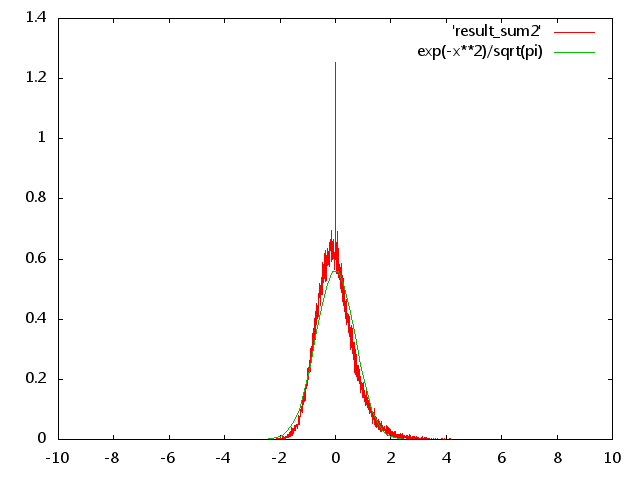
\includegraphics[width=4in]{sum2.png}
\end{center}
对 $Z = \frac{X_1+X_2+X_3}{3}$, 结果为:
\begin{center}
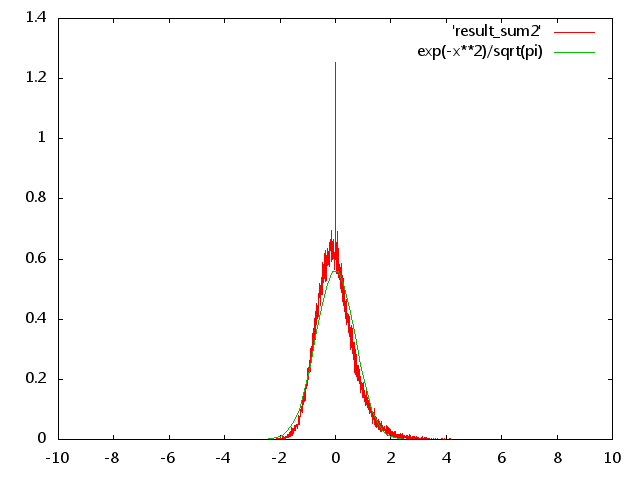
\includegraphics[width=4in]{sum2.png}
\end{center}
绿线是理论曲线, 可以看到, 和中心极限定理的结果是相当一致的.

\end{document}
